% !TEX TS-program = pdflatexmk
% !BIB TS-program = bibtex

\documentclass[12pt, a4paper, oneside]{book}
\usepackage{import}
\subimport{../}{preamble}
\ExecuteBibliographyOptions{articletitle=false}
\standalonetrue
\onehalfspacing
\begin{document}

\begin{singlespace}
\chapter{Electrochemical Fabrication of Spherical AuNP-Tipped AFM Probes}
\end{singlespace}

\AddToShipoutPictureBG*{ \AtPageUpperLeft{ \put(0,-260)
{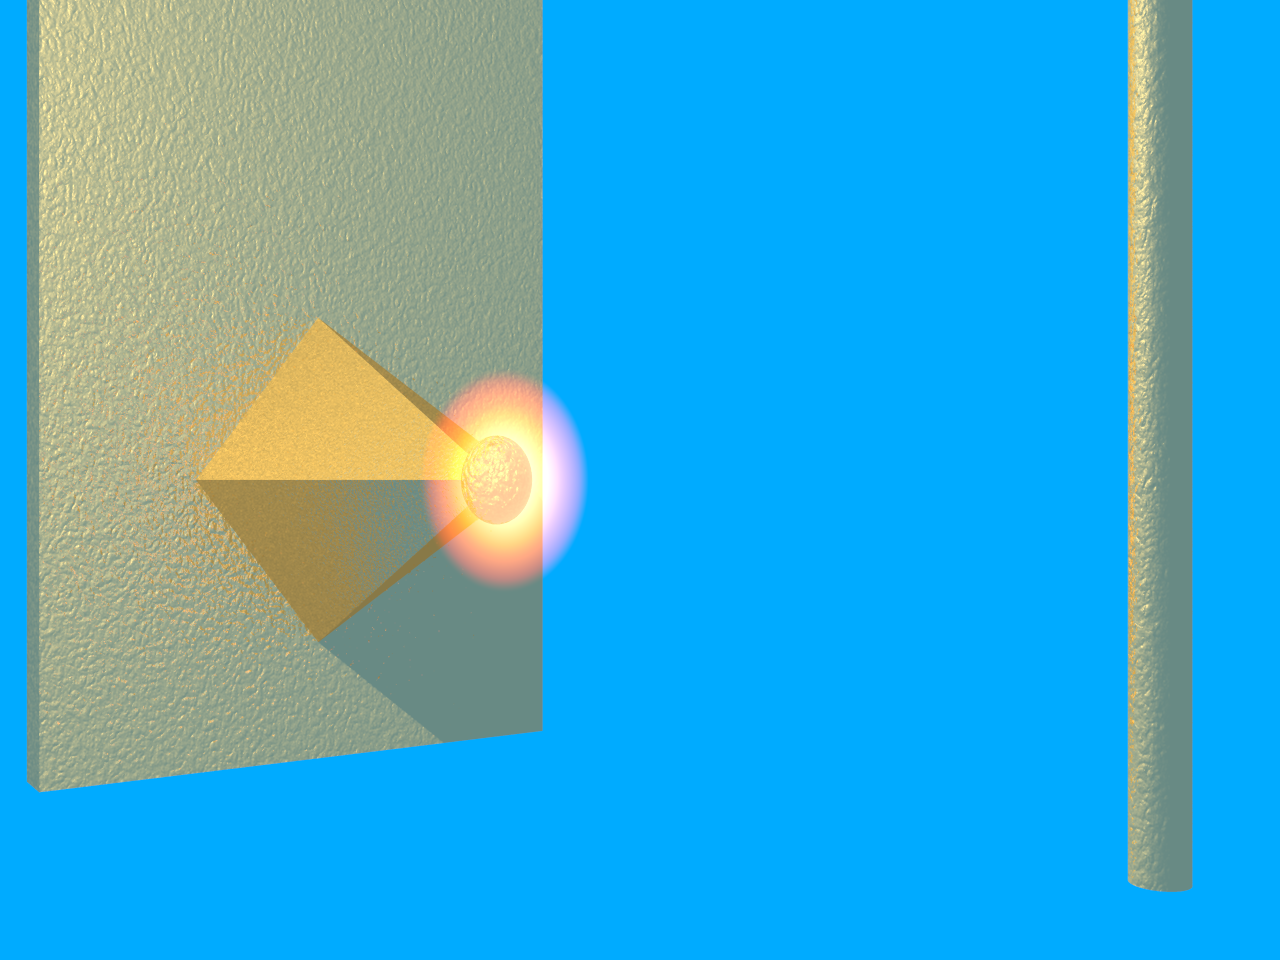
\includegraphics[width=\paperwidth, clip=true, trim=0 120 0 200]{data/chapter_cover.png}}
}}

As discussed in the previous chapter, nanostructuring a tip can create the necessary geometry and electromagnetic interfaces to support antenna-like plasmons. This enables coupling with far-field light and can improve the plasmonic performance of such tips. Consequently, this also means that excited plasmons scatter into the far-field and are therefore experimentally observable. This is a crucial property when using tips to measure fundamental plasmonics. Because of this, one of the major aims of this project is to produce robust nanostructured, plasmonic tips. The spherical geometry is targeted for its simplicity.

Fabrication of spherical tips has previously been achieved by mounting single nanoparticles onto the apices of tips. This concept has been reported numerous times over the last decade \cite{gan2007}, beginning with the use of fibres as mounting structures \cite{kalkbrenner2001, barsegova2002, sqalli2002, kawata2003} and progressing onto the use of \gls{spm} tips \cite{umakoshi2012, hayazawa2012, park2012, okamoto2001, vakarelski2006}. Whilst mounting nanoparticles onto \gls{spm} tips is more difficult than with fibres the additional capabilities of the SPM tip have made such tips desirable. However, these tips typically require complicated assembly processes to precisely secure a single \gls{np} at the apex of the tip, greatly increasing their fabrication time and costs. More recent methods have attempted to address the complexity issue by directly depositing nanoparticles onto the apex by exploiting localised chemical reactions. Nevertheless, these techniques have still been limited by cost or required specialist equipment \cite{sqalli2002, okamoto2001}, incompatible with SPM probes \cite{kharintsev2013, barsegova2002} or subject to limitations in nanoparticle growth, either in size \cite{cheng2013} or material \cite{umakoshi2012}.
Non-metallic spherical tips on \gls{afm} probes have been created using methods such as vacuum-processing diamond-like carbon growth (NanoTools B-series). These nanotips can then be made plasmonic through evaporation of a metallic coating.
%It remains a challenge to find a simple and efficient method for reliably producing spherical nanoparticle tips. Here we provide a simple and efficient method for reliably producing spherical nanoparticle tips using apex-selected electrochemical growth.
Even in recent years it still remains a challenge to simply and efficiently produce spherically nanostructured tips.

Electrochemical deposition is highly suited to the tip geometry because of the large d.c.\ field enhancement localised at the sharp apex point. Due to its significantly reduced radius of curvature, the equipotential surface resulting from an applied voltage leads to the compression of field lines at the tip apex. This strongly increases the field amplitude in the vicinity of the tip apex and is known as the lightning rod effect. Under such conditions the rate of electrochemical reactions is significantly increased around the tip apex. By exploiting this localised field enhancement it is possible to grow a spherical \gls{mnp} directly onto the tip apex. Whilst use of the lightning rod effect for electrochemical growth has been used to grow dense forests of \glspl{mnp} \cite{tian2006, yang2011} it has yet to be applied to the fabrication of single \glspl{mnp} at a tip's apex.

Selective growth of \glspl{mnp} onto the apices of tips is difficult using traditional methods of electrochemical deposition but can instead be achieved by using single-pulse, high-field electrochemical growth. This chapter describes the process of pulsed electrodeposition for apex-selective nucleation and growth of AuNP \gls{afm} tips. The process of electrochemistry is first described followed by discussion of the method by which spherical AuNP-tipped AFM probes are produced.
%A second method is then discussed, addressing the issues and limitations with the original method and circumventing them at the cost of production rate.

\subimport{./}{electrochemistry_theory}
\subimport{./}{initial_fabrication}
%\subimport{./}{modified_method}
\subimport{./}{post_processing}

\section{Conclusions}

By using electrochemical deposition, the simple fabrication of spherical metallic tips has been successfully demonstrated. Tips can be fabricated within a short period of time and with high throughput using pulsed electrochemical deposition, exploiting the sharp tip geometry to nucleate and grow a single nanoparticle at the apex. Though simple and cheap compared with many other techniques, control of growth morphology quality still presents issues. The many free variables in the system are problematic for morphology control and are yet to be fully understood and optimised. As a result, there is currently little ability to predict the size and shape of nanoparticles. Nevertheless, the deposition process succeeded in its original purpose of providing spherical AuNP tips for plasmonic applications that can be electrically contacted to measure charge transfer through a plasmonic nanogap.

Several advantages emerge from apex-selective single nanoparticle electrochemical growth. The capability for simultaneous nanoparticle growth on many tips ensures a high throughput process, while morphology and size is controlled by voltage and time. This provides a viable method for producing tips capable of expanding the user-base of plasmonics and furthering research into applications of TERS and SNOM. Furthermore, the spherical nanoparticle growth method introduced here is not restricted to specific metals, and many different composite systems can be created with this apex-localised growth technique. For example, silver nanoparticle tips could give a large optical response and field enhancement under visible illumination (although oxidation is sometimes an issue). This technique could therefore become a simple route to effectively improve TENOM across a broadband wavelength range.

\ifstandalone
\begin{singlespace}
\fontsize{8pt}{1em}\selectfont
\printbibliography[notcategory=fullcited]
\end{singlespace}
\fi

\end{document}